\chapter{ MARCO METODOLÓGICO}
% ======================================================================
% SECCION DE METODOLOGIA - Tesis Estela de Raimondi
% Texto listo para pegar en LaTeX. Citas con \cite{} (BibTeX, IEEEtran).
% Las claves de [1]-[50] son una PROPUESTA (autor+anio); ajustar a tu .bib
% (ver tabla de equivalencia al final). Las 5 entradas nuevas vienen como
% BibTeX listo para pegar. Sin guiones largos. Genes y especies en \textit{}.
% ======================================================================

\section{Metodología}

\subsection{Diseño general y criterios de decisión metodológica}

El estudio es de naturaleza estrictamente computacional y descriptiva. Parte de datos metagenómicos shotgun previamente secuenciados y ensamblados en el marco del informe técnico microbiológico de la Estela de Raimondi, realizado por UPCH \cite{tsukayama2025informe}, sobre los cuales se construye un flujo bioinformático que va desde el control de calidad de los genomas hasta la inferencia del potencial metabólico de los linajes dominantes. El flujo se organiza en cuatro fases consecutivas, cada una asociada a un objetivo específico (OE1 a OE4), y se ejecuta en el orden presentado a continuación.

\subsection{Origen de los datos y unidad de análisis}

%El microbioma de la Estela de Raimondi fue muestreado mediante hisopado en seco sobre la superficie del monumento. En cada punto de muestreo se recolectaron dos hisopados independientes: el hisopo A, destinado a la extracción directa de ADN ambiental para secuenciación de amplicones (16S rRNA e ITS2), y el hisopo B, destinado al cultivo microbiológico de la fracción viable \cite{tsukayama2025informe}. La secuenciación metagenómica shotgun analizada en esta tesis se realizó sobre el material proveniente del cultivo (hisopo B). En consecuencia, los genomas reconstruidos representan la fracción microbiana recuperable mediante cultivo y no necesariamente las poblaciones dominantes \textit{in situ}. Esta condición se trata de forma explícita como limitación en la Fase 3.

El microbioma de la Estela de Raimondi fue muestreado mediante hisopado en seco sobre la superficie del monumento. En cada punto de muestreo se recolectaron dos hisopados independientes: el hisopo A, destinado a la extracción directa de ADN ambiental para secuenciación de amplicones (16S rRNA e ITS2), y el hisopo B, destinado al cultivo microbiológico de la fracción viable \cite{tsukayama2025informe}. La secuenciación metagenómica shotgun analizada en esta tesis se realizó sobre el material proveniente del cultivo (hisopo B). 

\begin{figure}[H]
    \centering
    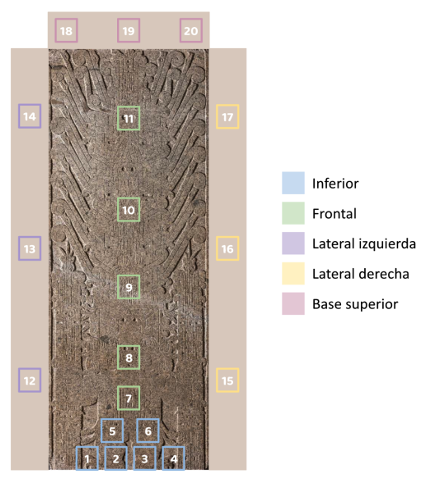
\includegraphics[width=0.8\textwidth]{images/Muestras.png}
    \caption{Esquema de muestreo de la Estela de Raimondi. Se señalan los 20 puntos de hisopado distribuidos sobre las cinco regiones del monumento (base superior, cara frontal, laterales izquierda y derecha, y sección inferior). En cada punto se recolectaron dos hisopados independientes: el hisopo A, destinado a la extracción directa de ADN para secuenciación de amplicones, y el hisopo B, destinado al cultivo de la fracción viable, posteriormente secuenciado por metagenómica \textit{shotgun}. Tomado del informe técnico de la UPCH~\cite{tsukayama2025informe}.}
    \label{fig:muestreo}
\end{figure}

Si bien la metagenómica suele aplicarse de
forma independiente de cultivo, en el estudio del patrimonio pétreo se han documentado
también aproximaciones dependientes de cultivo acopladas a la identificación molecular por
secuenciación~\cite{suchy2024}. En consecuencia, los genomas reconstruidos representan la fracción microbiana recuperable mediante cultivo y no necesariamente las poblaciones dominantes \textit{in situ}. Esta condición se trata de forma explícita como limitación en la Fase 3.


\begin{table}[htbp]
\centering
\small
\renewcommand{\arraystretch}{1.05}
\setlength{\tabcolsep}{3pt}
\caption{Bins genómicos recuperados por muestra (previos al filtrado por dominio y calidad).}
\label{tab:bins}

\makebox[\textwidth][c]{%
\begin{tabular}{c c c c c c}
\hline
\textbf{Muestra} & \textbf{N.\textsuperscript{o} bins} & \textbf{Long. total (Mb)} & \textbf{Rango bin (Mb)} & \textbf{N50 prom. (kb)} & \textbf{\%GC prom.} \\
\hline
49 & 2  & 28.1  & 0.55--27.6  & 173 & 36.2 \\
50 & 6  & 67.3  & 0.61--53.4  & 47  & 59.5 \\
51 & 1  & 4.7   & 4.73        & 189 & 52.6 \\
52 & 5  & 18.2  & 0.42--5.3   & 37  & 61.6 \\
53 & 3  & 36.9  & 2.48--29.2  & 264 & 40.5 \\
54 & 2  & 11.6  & 4.31--7.3   & 167 & 38.7 \\
55 & 1  & 34.2  & 34.24       & 404 & 51.1 \\
56 & 6  & 88.4  & 0.23--49.6  & 95  & 45.6 \\
57 & 6  & 74.7  & 0.22--39.1  & 164 & 46.9 \\
58 & 3  & 46.5  & 4.77--29.6  & 418 & 48.5 \\
59 & 2  & 29.1  & 5.91--23.2  & 283 & 40.9 \\
60 & 5  & 49.6  & 2.32--25.7  & 52  & 43.5 \\
61 & 6  & 73.1  & 0.61--40.1  & 207 & 47.7 \\
62 & 5  & 45.7  & 0.23--27.9  & 128 & 39.4 \\
63 & 6  & 88.8  & 0.37--56.5  & 40  & 45.7 \\
64 & 7  & 75.5  & 0.24--29.7  & 33  & 43.4 \\
65 & 5  & 94.8  & 0.22--29.6  & 89  & 47.0 \\
66 & 0  & ---   & ---         & --- & ---  \\
67 & 0  & ---   & ---         & --- & ---  \\
68 & 2  & 2.7   & 0.25--2.5   & 43  & 49.2 \\
69 & 2  & 2.7   & 0.25--2.5   & 40  & 49.1 \\
70 & 6  & 109.2 & 0.28--94.3  & 3   & 44.0 \\
71 & 12 & 126.9 & 0.26--101.9 & 6   & 47.2 \\
72 & 4  & 9.7   & 0.25--6.6   & 4   & 38.9 \\
\hline
\textbf{Total} & \textbf{97} & & & & \\
\hline
\end{tabular}%
}

\vspace{0.5em}

\begin{minipage}{0.95\textwidth}
\footnotesize
\textit{Nota.} Se dispuso de 24 librerías de secuenciación Illumina, identificadas con los códigos 49 a 72. El procesamiento previo, documentado por el centro de secuenciación, comprendió el ensamblaje por muestra mediante MEGAHIT, la segmentación del ensamblaje en bins genómicos mediante MetaBAT2, la evaluación de métricas de ensamblaje con QUAST y la anotación preliminar de cada bin con Bakta, junto con una asignación taxonómica preliminar basada en Kraken2. Un bin corresponde, en este punto del flujo, a un subconjunto de contigs del ensamblaje agrupados según su perfil de cobertura y composición de tetranucleótidos, bajo el supuesto de que los contigs pertenecientes a un mismo organismo comparten estas señales. Por tanto, cada bin constituye una reconstrucción parcial o completa de un genoma individual, cuya pureza taxonómica y calidad genómica se evalúan posteriormente. De las 24 librerías, 22 produjeron bins, con un total de 97 bins; las muestras 66 y 67 no recuperaron bins y fueron excluidas del análisis genómico. Las cifras mostradas corresponden a bins crudos entregados por el centro de secuenciación y preceden al filtrado por dominio y al control de calidad genómica descritos en la Fase 1; por ello, no implican que la totalidad de los bins listados sean genomas procariotas completos o libres de contaminación.
\end{minipage}

\end{table}
Las lecturas crudas (archivos FASTQ) no estuvieron disponibles para este
trabajo. Por ello, todo el flujo se ejecuta sobre los genomas ensamblados
(bins) y no sobre lecturas. En consecuencia, la importancia de cada linaje no
se mide por abundancia, sino por prevalencia espacial: el número de puntos de
muestreo distintos en los que se recuperó ese linaje. Esta métrica no depende
de las lecturas crudas y es más robusta frente al sesgo del cultivo.


\subsection{Fase 1. Control de calidad y selección de genomas (OE1)}

\subsubsection{Filtrado por dominio}

Los bins se filtraron primero por dominio para descartar contigs de origen eucariota u organelar antes de cualquier métrica basada en genes procariotas. Se utilizó Tiara \cite{karlicki2022tiara}, un clasificador de secuencias metagenómicas basado en aprendizaje profundo que opera sobre la composición de los contigs en un esquema de dos etapas. La elección de Tiara frente a Whokaryote \cite{pronk2022whokaryote} y EukRep \cite{west2018genomereconstruction} se sustentó en la matriz de selección ponderada (Tabla~\ref{tab:seleccion_software}), en la que Tiara obtuvo la mayor puntuación total gracias a su facilidad de instalación, su menor costo computacional y su capacidad adicional de identificar ADN organelar; la descripción detallada de cada herramienta evaluada se presenta en el Anexo 1.

\begin{table}[H]
\centering
\footnotesize
\caption{Matriz de selección de software para la clasificación de contigs.}
\label{tab:seleccion_software}
\begin{tabular}{@{}lcccccccc@{}}
\toprule
& & \multicolumn{2}{c}{\textbf{Tiara}} & \multicolumn{2}{c}{\textbf{Whokaryote}} & \multicolumn{2}{c}{\textbf{EukRep}} \\
\cmidrule(lr){3-4} \cmidrule(lr){5-6} \cmidrule(lr){7-8}
\textbf{Criterio} & \textbf{Peso (\%)} & \textbf{Pts} & \textbf{Peso$\times$Pts} & \textbf{Pts} & \textbf{Peso$\times$Pts} & \textbf{Pts} & \textbf{Peso$\times$Pts} \\
\midrule
Facilidad de instalación & 10 & 4 & 40 & 3 & 30 & 2 & 20 \\
Acceso a dependencias & 15 & 4 & 60 & 2 & 30 & 2 & 30 \\
Costo computacional & 10 & 3 & 30 & 2 & 20 & 3 & 30 \\
Integración en pipeline & 15 & 4 & 60 & 3 & 45 & 2 & 30 \\
Calidad de resultado & 30 & 4 & 120 & 3 & 90 & 2 & 60 \\
Alcance funcional & 10 & 4 & 40 & 2 & 20 & 2 & 20 \\
Interpretabilidad & 10 & 3 & 30 & 4 & 40 & 2 & 20 \\
\midrule
\textbf{Total} & \textbf{100} & & \textbf{380} & & \textbf{275} & & \textbf{210} \\
\bottomrule
\end{tabular}
\end{table}

Se aplicó una longitud mínima de contig de 3000 pares de bases, valor por debajo del cual los clasificadores basados en composición de secuencia pierden exactitud, y se descartaron los bins cuya fracción mayoritaria de longitud se clasificó como eucariota u organelar. Dado que Tiara discrimina entre procariotas y eucariotas pero no separa bacterias de arqueas, esta última distinción se resolvió en las fases posteriores mediante CheckM2 y GTDB-Tk.


\subsubsection{Evaluación de la calidad genómica}

La completitud y la contaminación de los bins procariotas se estimaron con CheckM2 \cite{checkm2}, que predice ambas métricas mediante modelos de aprendizaje automático entrenados sobre genomas de referencia y no requiere asignación taxonómica previa, lo que mejora su desempeño en linajes divergentes \cite{checkm2}. Se conservaron únicamente los genomas con completitud superior al 70\% y contaminación inferior al 5\%.

El umbral no corresponde a ninguna categoría MIMAG estándar. Se adoptó un valor intermedio que flexibiliza la exigencia de completitud, con el fin de recuperar genomas ambientales fragmentados, pero mantiene la restricción más estricta de contaminación (inferior al 5\%) para evitar que la posterior reconstrucción del genoma accesorio se sesgue por la inclusión de ADN foráneo \cite{bowers2017}. Este compromiso se documenta como criterio propio del proyecto y no como un estándar MIMAG de alta calidad.

\subsection{Fase 2. Asignación taxonómica y definición de linajes (OE2)}

\subsubsection{Clasificación taxonómica genómica}

Los genomas que superaron el control de calidad se clasificaron taxonómicamente con GTDB-Tk \cite{gtdbtk2019}, empleando los conjuntos de marcadores bac120 para bacterias y arc122 para arqueas. GTDB-Tk ubica cada genoma en el árbol de referencia del GTDB, que normaliza los rangos taxonómicos según la divergencia evolutiva relativa \cite{gtdbtk2019, gtdb2022}. Este enfoque basado en el genoma completo reemplaza a la asignación preliminar por Kraken2, de naturaleza basada en lecturas, por una clasificación de mayor resolución y consistencia filogenética.

\subsubsection{Confirmación de especie por ANI}

La clasificación de GTDB-Tk asigna taxonomía comparando características genómicas globales, pero no compara directamente el genoma completo contra una cepa de referencia. Para confirmar la identidad a nivel de especie, se calculó la Identidad Nucleotídica Promedio (ANI) entre cada genoma ensamblado y el genoma de referencia oficial de su taxón asignado. Este genoma de referencia corresponde a la cepa tipo de la especie (el organismo depositado en bases de datos públicas cuando esa especie fue descrita por primera vez, y que actualmente actúa como estándar de comparación).

El ANI mide qué tan parecidas son dos secuencias de ADN a lo largo del genoma completo. Dos genomas se consideran de la misma especie cuando el ANI es igual o superior al 95\% y al menos el 65\% del genoma puede alinearse \cite{fastANI2018, gtdbtk2019}.

\subsubsection{Desreplicación y definición de linajes}

Dado que el ensamblaje y el binning se realizaron por muestra de forma independiente, un mismo organismo presente en varias muestras pudo recuperarse como bins redundantes. Para colapsar esta redundancia se aplicó dRep  \cite{olm2017}, que agrupa los genomas en clústeres según su Identidad Nucleotídica Promedio (ANI). Se utilizó un umbral primario del 95\% de ANI para delimitar clústeres a nivel de especie, congruente con el radio de circunscripción taxonómica estándar empleado por la base de datos GTDB \cite{gtdbtk2019}. De forma complementaria, el agrupamiento secundario se definió a un umbral estricto del 99\% de ANI para lograr una resolución de cepa. Este último umbral permite agrupar genomas casi idénticos \cite{olm2017}, asegurando la desreplicación de poblaciones clonales sin colapsar cepas de la misma especie que pudieran albergar variaciones intraespecíficas relevantes. Cada clúster resultante se define operativamente como un linaje.

La desreplicación cumple dos funciones determinantes. Primero, provee varios genomas de la Estela por linaje, lo que habilita la construcción de un pangenoma interno con réplicas reales en la Fase 4. Segundo, permite definir una métrica de prevalencia objetiva, calculada como el número de muestras, sobre el total de 24, que aportan al menos un genoma a cada clúster. Esta métrica no depende de las lecturas crudas y por ello constituye el criterio primario de importancia de un linaje.

\subsubsection{Confirmación filogenómica}

La ubicación de cada linaje se visualizó mediante un árbol filogenómico focalizado que incluyó los genomas de la Estela y los genomas de referencia, inferido de novo por GTDB-Tk \cite{gtdbtk2019} a partir de los mismos marcadores bac120 empleados en la clasificación taxonómica. Esta elección, frente a la alternativa de inferir el árbol externamente con IQ-TREE \cite{minh2020}, se sustentó en la matriz de selección ponderada (Tabla~\ref{tab:seleccion_filogenomica}), en la que GTDB-Tk obtuvo la mayor puntuación gracias a su integración directa en el flujo ya ejecutado y a su menor costo computacional, criterio priorizado dada la restricción de cómputo propia de un proyecto de pregrado. Como contrapartida, el árbol de novo de GTDB-Tk no provee selección de modelo de sustitución ni soporte de rama mediante bootstrap, por lo que la topología resultante se interpreta como una verificación visual de la monofilia de cada linaje frente a las referencias, y no como una confirmación con soporte estadístico cuantificado.

\begin{table}[H]
\centering

\caption{Matriz de selección de software para la confirmación filogenómica.}
\label{tab:seleccion_filogenomica}

\resizebox{\textwidth}{!}{
\begin{tabular}{@{}lcccccc@{}}
\toprule
& & \multicolumn{2}{c}{\textbf{GTDB-Tk (árbol de novo)}} & \multicolumn{2}{c}{\textbf{IQ-TREE}} \\
\cmidrule(lr){3-4} \cmidrule(lr){5-6}
\textbf{Criterio} & \textbf{Peso (\%)} & \textbf{Pts} & \textbf{Peso$\times$Pts} & \textbf{Pts} & \textbf{Peso$\times$Pts} \\
\midrule
Facilidad de instalación & 20 & 4 & 80 & 3 & 60 \\
Acceso a dependencias & 20 & 4 & 80 & 3 & 60 \\
Costo computacional & 15 & 4 & 60 & 2 & 30 \\
Integración en pipeline & 20 & 4 & 80 & 3 & 60 \\
Calidad de resultado & 10 & 2 & 20 & 4 & 40 \\
Alcance funcional & 5  & 2 & 10 & 4 & 20 \\
Interpretabilidad & 10 & 2 & 20 & 4 & 40 \\
\midrule
\textbf{Total} & \textbf{100} & & \textbf{350} & & \textbf{310} \\
\bottomrule
\end{tabular}
}
\end{table}

\subsubsection{Selección de linajes para el análisis comparativo}

A partir de los linajes definidos, entendidos como los clústeres de especie obtenidos al 95\% de ANI, se priorizaron los de mayor prevalencia. Por restricciones de cómputo, el análisis comparativo se concentró en los tres linajes de mayor prevalencia. Para esta selección,  no se utilizó la abundancia de secuencias, ya que los cultivos previos en laboratorio sesgan estos números. En su lugar, se utilizó el criterio de \textbf{prevalencia espacial} \cite{olm2017}. Esto consistió en seleccionar a las especies que lograron ser ensambladas en la mayor cantidad de puntos físicos distintos de la Estela Raimondi. La detección repetida de un mismo genoma a través de múltiples muestras independientes demuestra que se trata de microorganismos residentes y estables, y no de simple polvo o contaminación ambiental

Esta elección de la especie como unidad primaria de análisis resulta indispensable para el correcto funcionamiento de Panaroo, dado que el algoritmo requiere comparar un conjunto de genomas estrechamente emparentados para diferenciar con precisión los genes esenciales y conservados (genoma core) de aquellos genes ganados o perdidos como producto de la adaptación evolutiva al nicho específico (genoma accesorio). Cuando la comparación se realiza entre genomas filogenéticamente distantes, esta distinción pierde fiabilidad, pues la divergencia de secuencia entre especies no relacionadas introduce una subestimación artificial del genoma core, atribuible a limitaciones del método de detección de ortólogos y no a una reducción real del repertorio génico compartido \cite{panaroo2020}.

%\subsection{Fase 3. Validación cruzada con el perfil ambiental 16S}

%Para evaluar la relevancia ecológica de los linajes recuperados de la fracción cultivable, su composición se contrastó con el perfil taxonómico de la comunidad ambiental total. Este perfil proviene de la secuenciación de amplicones 16S rRNA del hisopo A, procesada en el informe técnico previo frente a la base de datos SILVA \cite{tsukayama2025informe}. La comparación se realizó a nivel de género: la presencia, y en particular la abundancia, de los géneros seleccionados en el perfil ambiental se interpreta como evidencia de que dichos linajes son miembros genuinos de la comunidad colonizadora y no errores del cultivo. Dado que la taxonomía de SILVA y la del GTDB no son equivalentes, los nombres de género se armonizaron entre ambos sistemas antes de la comparación. Este paso convierte la limitación impuesta por el origen cultivado de la muestra en un control de relevancia ecológica.

\subsection{Fase 3. Análisis pangenómico comparativo (OE3)}

\subsubsection{Recopilación de genomas de referencia}

Para cada uno de los tres linajes seleccionados se recopilaron genomas de referencia desde NCBI RefSeq y GTDB. Se incluyeron genomas de la especie asignada por GTDB-Tk y, cuando el número de referencias a nivel de especie fue insuficiente, se amplió al género correspondiente. Se priorizaron los ensamblajes designados como completos o representativos en RefSeq, que ya han pasado por el proceso de curación de NCBI. Cuando un linaje no contó con referencias de especie en RefSeq, se recurrió a los genomas tipo de GTDB como alternativa.

El conjunto de referencias se desreplicó con dRep a un umbral del 99\% de ANI, con el fin de evitar que genomas casi clonales, frecuentes en taxones muy secuenciados, inflaran artificialmente el genoma núcleo. El número de genomas de referencia no se fijó de forma arbitraria, sino que se determinó mediante la curva de acumulación del pangenoma: se añadieron genomas secuencialmente hasta observar la estabilización del genoma núcleo \cite{tettelin2005}. Cuando un taxón presentó menos de aproximadamente diez genomas de referencia de calidad suficiente en bases de datos públicas, el conjunto se amplió siguiendo el mismo criterio. En el caso de los linajes arqueales, para los que la disponibilidad de referencias de calidad fue menor, el linaje se incluyó en el análisis comparativo solo si reunió genomas suficientes para estabilizar la curva; en caso contrario, se describió de forma individual sin pangenoma comparativo.

\subsubsection{Anotación estructural y funcional consistente}

La totalidad de los genomas, tanto los MAGs de la Estela como las referencias, se anotó con la misma herramienta y versión para garantizar la homogeneidad requerida por el análisis pangenómico \cite{panaroo2020}. Se empleó Bakta \cite{schwengers2021}, que realiza la predicción de marcos abiertos de lectura y la anotación mediante identificación de secuencias sin alineamiento, y que ya se había aplicado a los bins originales. Esta elección, frente a la alternativa de Prokka \cite{prokka2014} (heredero directo de Prodigal \cite{Hyatt2010}), se sustentó en la matriz de selección ponderada (Tabla~\ref{tab:seleccion_anotacion}), en la que Bakta obtuvo la mayor puntuación gracias a su continuidad con la anotación ya aplicada a los bins originales, su mayor resolución en linajes ambientales divergentes y su alcance funcional más amplio; Prokka resultó más liviano de instalar, pero con menor calidad de resultado en MAGs poco representados en bases de datos curadas. La anotación consistente evita que diferencias en la predicción génica se confundan con diferencias biológicas.

\begin{table}[H]
\centering
\footnotesize
\caption{Matriz de selección de software para la anotación estructural y funcional.}
\label{tab:seleccion_anotacion}
\begin{tabular}{@{}lcccccc@{}}
\toprule
& & \multicolumn{2}{c}{\textbf{Bakta}} & \multicolumn{2}{c}{\textbf{Prokka}} \\
\cmidrule(lr){3-4} \cmidrule(lr){5-6}
\textbf{Criterio} & \textbf{Peso (\%)} & \textbf{Pts} & \textbf{Peso$\times$Pts} & \textbf{Pts} & \textbf{Peso$\times$Pts} \\
\midrule
Facilidad de instalación & 10 & 3 & 30  & 4 & 40 \\
Acceso a dependencias    & 10 & 3 & 30  & 4 & 40 \\
Costo computacional      & 5  & 3 & 15  & 4 & 20 \\
Integración en pipeline  & 25 & 4 & 100 & 2 & 50 \\
Calidad de resultado     & 25 & 4 & 100 & 2 & 50 \\
Alcance funcional        & 15 & 4 & 60  & 3 & 45 \\
Interpretabilidad        & 10 & 4 & 40  & 3 & 30 \\
\midrule
\textbf{Total} & \textbf{100} & & \textbf{375} & & \textbf{275} \\
\bottomrule
\end{tabular}
\end{table}

\subsubsection{Reconstrucción del pangenoma}

El pangenoma de cada linaje se reconstruyó con Panaroo \cite{panaroo2020} en su modo estricto (clean-mode strict). Esta elección, frente a la alternativa de PPanGGOLiN \cite{ppanggolin2020}, se sustentó en la matriz de selección ponderada (Tabla~\ref{tab:seleccion_pangenoma}), en la que Panaroo obtuvo la mayor puntuación gracias a su representación gráfica del pangenoma, que corrige errores de anotación y de ensamblaje mediante la propagación del contexto genómico vecino y reduce de forma marcada la inflación artificial del genoma accesorio asociada a la fragmentación de los MAGs; PPanGGOLiN, pese a ofrecer un modelo probabilístico de partición con módulos adicionales (regiones de plasticidad genómica), no corrige esta inflación con la misma eficacia en colecciones de MAGs fragmentados.

\begin{table}[H]
\centering
\footnotesize
\caption{Matriz de selección de software para la reconstrucción del pangenoma.}
\label{tab:seleccion_pangenoma}
\begin{tabular}{@{}lcccccc@{}}
\toprule
& & \multicolumn{2}{c}{\textbf{Panaroo}} & \multicolumn{2}{c}{\textbf{PPanGGOLiN}} \\
\cmidrule(lr){3-4} \cmidrule(lr){5-6}
\textbf{Criterio} & \textbf{Peso (\%)} & \textbf{Pts} & \textbf{Peso$\times$Pts} & \textbf{Pts} & \textbf{Peso$\times$Pts} \\
\midrule
Facilidad de instalación & 10 & 3 & 30  & 3 & 30 \\
Acceso a dependencias    & 10 & 3 & 30  & 3 & 30 \\
Costo computacional      & 5  & 3 & 15  & 4 & 20 \\
Integración en pipeline  & 15 & 3 & 45  & 3 & 45 \\
Calidad de resultado     & 35 & 4 & 140 & 2 & 70 \\
Alcance funcional        & 15 & 3 & 45  & 4 & 60 \\
Interpretabilidad        & 10 & 4 & 40  & 3 & 30 \\
\midrule
\textbf{Total} & \textbf{100} & & \textbf{345} & & \textbf{285} \\
\bottomrule
\end{tabular}
\end{table}

El pangenoma se particionó en tres compartimentos siguiendo la convención de la genómica comparativa \cite{panaroo2020, tettelin2005, Page2015}: genoma nuclear (genes presentes en al menos el 95\% de los genomas), genoma de cubierta o shell (genes en el 15 a 95\%) y genoma accesorio o cloud (genes en menos del 15\%).

\subsubsection{Identificación de genes candidatos exclusivos de la Estela}

Los genes candidatos a ser exclusivos de la Estela se definieron como aquellos presentes en uno o más MAGs del monumento y ausentes en todos los genomas de referencia. Para reducir la probabilidad de errores, se exigió que el gen estuviera completo y no truncado en el borde de un contig. Los candidatos se contrastaron mediante búsqueda de homología frente a las bases de datos nr (non-redundant) y nt (nucleotide) para descartar contaminación. Estos genes se interpretan en el marco de la transferencia horizontal de genes como principal motor de adaptación ecológica en procariotas \cite{soucy2015}. Dado que la incompletitud de los MAGs implica que la ausencia observada de un gen no equivale a su ausencia real \cite{bowers2017}, los resultados se reportan como candidatos a exclusivos y como adquisición probable, sin afirmar certeza.

\subsection{Fase 4. Caracterización del potencial metabólico y del riesgo (OE4)}

\subsubsection{Anotación funcional del potencial metabólico}


El potencial metabólico de los linajes seleccionados se caracterizó con la herramienta DRAM \cite{dram2020}, la cual integra la asignación de ortólogos KEGG (KO) y produce resúmenes de los ciclos biogeoquímicos del nitrógeno, el azufre y el carbono, así como el inventario de enzimas activas sobre carbohidratos (CAZymes) basado en las bases dbCAN y CAZy. Para la evaluación de los módulos de KEGG, DRAM modela las vías como redes dirigidas y calcula la completitud como el porcentaje de cobertura de la ruta que presenta la mayor proporción de genes (nodos) detectados \cite{dram2020}. Sobre esta base, en el presente estudio se estableció un umbral operativo estricto: un módulo metabólico se consideró funcionalmente "presente" solo cuando su porcentaje de completitud alcanzó o superó el 66\%. Para las funciones que dependen de varios genes, la presencia se definió mediante una regla explícita para cada función, descrita en la Tabla~\ref{tab:marcadores}.

\subsubsection{Definición de marcadores de riesgo y supervivencia}

La interpretación funcional se ancló en una tabla de marcadores genómicos definida \textit{a priori}, es decir, fijada antes de observar los resultados, con el fin de evitar el sesgo de confirmación. Cada marcador corresponde a una función y no a un gen aislado, de modo que una función que requiere varios genes se cuenta una sola vez. La tabla organiza las funciones en tres categorías. La primera reúne los marcadores de riesgo de biodeterioro: la producción de ácido glucónico y de ácido 2-cetoglucónico, que acidifican el sustrato y actúan como quelantes de silicatos \cite{gutarowska2015}; la biosíntesis de sustancias poliméricas extracelulares (EPS) y la adhesión mediante curli, que sostienen la biopelícula \cite{flemming2010}; y la nitrificación y la oxidación del azufre como fuentes de ácidos inorgánicos \cite{dakal2012, zanardini2019}. La segunda reúne los marcadores de supervivencia o persistencia: la esporulación \cite{Galperin2022}, la síntesis de carotenoides, la respuesta al estrés oxidativo, la síntesis de los solutos compatibles ectoína y trehalosa, que protegen frente a la desecación, y la reparación del ADN dañado por radiación ultravioleta. La tercera reúne funciones de contexto que se reportan pero no se interpretan como marcadores de riesgo: el ciclo de los ácidos tricarboxílicos, presente en prácticamente todas las bacterias aerobias \cite{zanardini2019}, las enzimas activas sobre carbohidratos (CAZymes) \cite{cantarel2009,zhang2018} y la ureólisis, cuya precipitación de carbonato puede tanto proteger como alterar la superficie pétrea.

La Tabla~\ref{tab:marcadores} detalla, para cada función, los genes representativos, sus identificadores KEGG Orthology (KO) y la regla con la que se considera presente. Las reglas exigen los genes necesarios para que la función sea operativa. Por ejemplo, la glucosa deshidrogenasa \textit{gcd} solo se cuenta como productora de ácido glucónico si el genoma porta además los genes de síntesis de su cofactor, la pirroloquinolina quinona (\textit{pqqA}--\textit{E}). Del mismo modo, la nitrificación y la oxidación del azufre se evalúan con los módulos KEGG completos (M00528 y M00595) y no con genes aislados. Los genes cuya función no distingue el proceso de interés se excluyeron: la nitrato reductasa \textit{narG} comparte identificador KO con la nitrito oxidorreductasa \textit{nxrA}, y la sulfito reductasa disimilatoria \textit{dsrAB} participa tanto en la reducción como en la oxidación del azufre. Los identificadores KO y los módulos se verificaron directamente contra la base de datos KEGG \cite{kegg2023}. Las CAZymes no poseen un identificador KO único; su detección se realiza mediante la base de datos dbCAN, integrada en DRAM. La detección efectiva de cada función en los genomas se obtiene de DRAM durante la fase de anotación funcional.

\subsubsection{Integración del potencial funcional con la estructura del pangenoma}

En el paso final, cada marcador de la tabla \textit{a priori} se mapeó sobre la partición del pangenoma para determinar si reside en el genoma nuclear o en el accesorio. Para evaluar de forma cuantitativa si los marcadores de riesgo se concentran en el genoma accesorio, se aplicó una prueba exacta de Fisher sobre una tabla de contingencia de dos por dos que cruza la condición de gen de riesgo o no de riesgo con su pertenencia al genoma accesorio o nuclear, reportando tanto el valor de probabilidad como la razón de momios (odds ratio) como medida del tamaño del efecto. Cuando se evaluaron varias categorías funcionales de forma simultánea, los valores de probabilidad se ajustaron por comparaciones múltiples mediante el procedimiento de Benjamini y Hochberg. Esta prueba se interpreta con cautela por dos razones: las familias génicas no constituyen observaciones estadísticamente independientes, debido a la no independencia filogenética, y el número reducido de marcadores de riesgo limita la potencia estadística. Por ello, el resultado se presenta como evidencia de apoyo y no como prueba concluyente. De forma complementaria, se caracterizó la apertura del pangenoma estimando el parámetro de la ley de Heaps \cite{ppanggolin2020}.

La lógica interpretativa es la siguiente. Si los genes de biodeterioro se enriquecen de forma significativa en el genoma accesorio, en particular si son compartidos por varios MAGs del mismo linaje, ello aporta soporte cuantitativo a la hipótesis de que dichas funciones fueron adquiridas como adaptación al nicho del monumento. Si, por el contrario, residen en el genoma nuclear, se interpretan como rasgos intrínsecos y conservados del linaje. En coherencia con el alcance del estudio, estas conclusiones describen el potencial metabólico codificado y no la actividad biológica real en el momento del muestreo.

% Requiere en el preambulo: \usepackage{tabularx}
% Si el documento es a dos columnas (p. ej. IEEEtran) y la tabla queda muy
% apretada, cambia \begin{table} por \begin{table*} para que ocupe el ancho
% completo de la pagina.
\newcolumntype{Q}[1]{>{\hsize=#1\hsize\raggedright\arraybackslash}X}
\begin{table*}[htbp]
\centering
\footnotesize
\setlength{\tabcolsep}{4pt}
\caption{Marcadores genómicos \textit{a priori} de biodeterioro, supervivencia y contexto, con la regla de presencia de cada función.}
\label{tab:marcadores}
% Fuente de trabajo: metadata/marcadores_fase4.tsv del repositorio del pipeline.
% KO y modulos verificados contra la API de KEGG (rest.kegg.jp) el 06-10-2026.
\begin{tabularx}{\linewidth}{Q{0.9} Q{1.1} Q{0.9} Q{1.3} Q{1.1} Q{0.7}}
\hline
\textbf{Categoría} & \textbf{Función / mecanismo} & \textbf{Genes} & \textbf{KO} & \textbf{Regla de presencia} & \textbf{Fuente} \\
\hline
Riesgo & Ácido glucónico (acidólisis y quelación) & gcd; pqqA--E & K00117; K06135--K06139 & gcd y al menos 3 de 5 genes pqq & \cite{gutarowska2015} \\
Riesgo & Ácido 2-cetoglucónico (quelación de silicatos) & gcd; pqqA--E; gluconato 2-deshidrogenasa & K00117; K06135--K06139; K06150, K06151, K06152 & regla anterior y al menos 2 de 3 subunidades & \cite{gutarowska2015} \\
Riesgo & EPS de biopelícula (Gram positivas) & epsA--O; tasA, tapA & K19419--K19431; K06336, K19433 & al menos 66\% del operón eps, o tasA y tapA & \cite{flemming2010} \\
Riesgo & EPS de biopelícula (Gram negativas) & pgaA, pgaB, pgaC, pgaD & K11935, K11931, K11936, K11937 & al menos 3 de 4 & \cite{flemming2010} \\
Riesgo & Adhesión (curli) & csgA, csgB & K04334, K04335 & ambos & \cite{flemming2010} \\
Riesgo & Nitrificación (ácido nítrico) & amoA, amoB, amoC, hao & K28504, K10945, K10946, K10535 & módulo M00528 al 66\% (3 de 4) & \cite{zanardini2019, dram2020} \\
Riesgo & Oxidación de azufre (ácido sulfúrico) & soxA, soxX, soxY, soxZ, soxB, soxC, soxD & K17222--K17227, K22622 & módulo M00595 al 66\% (5 de 7) & \cite{zanardini2019} \\
\hline
Supervivencia & Esporulación (latencia y resistencia) & spo0A, spoIIAA, spoIIE & K07699, K06378, K06382 & al menos 2 de 3 & \cite{Galperin2022} \\
Supervivencia & Carotenoides (protección UV) & crtB, crtI & K02291 o K17841; K10027 o K15745 & módulo M00097: crtB y crtI & \cite{basile2025} \\
Supervivencia & Estrés oxidativo & katA, sodA, dps & K03781, K04564, K04047 & al menos 2 de 3 & \cite{alonso2025, basile2025} \\
% TODO: verificar que alonso2025 y basile2025 respaldan ectoina, trehalosa y fotoliasas, o agregar fuentes especificas.
Supervivencia & Desecación: ectoína & ectA, ectB, ectC & K06718, K00836, K06720 & al menos 2 de 3 & \cite{alonso2025, basile2025} \\
Supervivencia & Desecación: trehalosa & otsA, otsB & K00697, K01087 & ambos & \cite{alonso2025, basile2025} \\
Supervivencia & Reparación del daño UV & fotoliasas (phr) & K01669, K06876 & al menos 1 & \cite{basile2025} \\
\hline
Contexto & Ácidos orgánicos del ciclo TCA & gltA, acnA, icd, sdhA, fumA & K01647, K01681, K00031, K00239, K01676 & módulo M00009 (descriptivo) & \cite{zanardini2019, gutarowska2015} \\
Contexto & CAZymes (polisacáridos) & familias GH, GT & sin KO único (dbCAN) & conteo por familia (descriptivo) & \cite{cantarel2009, zhang2018} \\
% TODO: agregar una fuente para la ureolisis y la precipitacion de carbonato.
Contexto & Ureólisis (precipitación de carbonato) & ureA, ureB, ureC & K01430, K01429, K01428 & los tres (descriptivo) & --- \\
\hline
\end{tabularx}
\end{table*}


\subsection{Reproducibilidad}
Se registró la versión exacta de cada herramienta bioinformática y la versión de cada base de datos empleada, y cada identificador KO se verificó contra la versión vigente de KEGG. El conjunto de software comprende, en orden de ejecución, Tiara \cite{karlicki2022tiara}, CheckM2 \cite{checkm2}, GTDB-Tk \cite{gtdbtk2019}, FastANI \cite{fastANI2018}, dRep \cite{olm2017}, Bakta \cite{schwengers2021}, Panaroo \cite{panaroo2020} y DRAM \cite{dram2020}. Las pruebas estadísticas se ejecutaron en un entorno de R con las bibliotecas correspondientes.

Los análisis computacionalmente intensivos se ejecutaron en el clúster de cómputo de alto rendimiento Khipu de la Universidad de Ingeniería y Tecnología (UTEC), modalidad Tesis. Este tipo de acceso permite el uso de las particiones \texttt{debug}, \texttt{debug-gpu}, \texttt{standard}, \texttt{gpu} y \texttt{big-mem}, con una asignación máxima por usuario de 32 núcleos de CPU, 98 GB de memoria RAM y 40 \textit{GPU shards}, además de un tiempo máximo de ejecución de 24 horas por trabajo computacional. La disponibilidad de esta infraestructura permitió ejecutar de manera controlada y reproducible las etapas de filtrado, evaluación de calidad, clasificación taxonómica, comparación genómica, anotación funcional y análisis pangenómico.

Para asegurar la trazabilidad del flujo de trabajo, se conservaron los comandos utilizados, los parámetros de ejecución, los archivos de entrada y salida, y los registros generados por cada herramienta. Asimismo, los resultados intermedios relevantes fueron organizados por etapa del análisis. Esta estructura permite auditar cada paso del procesamiento, repetir los análisis bajo las mismas condiciones computacionales y vincular los resultados finales con los archivos originales.


